\subsection{Протокол Wide-Mouth Frog}\index{протокол!Wide-Mouth Frog|(}
Протокол Wide-Mouth Frog является, возможно, самым простым протоколом с доверенным центром. Его автором считается Майкл Бэрроуз (1989 год, \langen{Michael Burrows},  \cite{Burrows:Abadi:Needham:1990}). Протокол состоит из следующих шагов.

\begin{figure}[!htb]
    \centering
    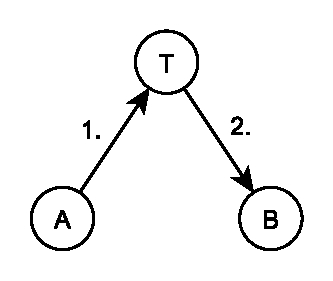
\includegraphics[width=0.5\textwidth]{pic/key_distribution-wide-mouth_frog}
    \caption{Схема взаимодействия абонентов и доверенного центра в протоколе Wide-Mouth Frog\label{fig:key_distribution-wide-mouth_frog}}
\end{figure}

\begin{enumerate}
	\item Алиса генерирует новый сеансовый ключ $K$ и отправляет его вместе с меткой времени, идентификатором Боба и своим незашифрованным идентификатором доверенному центру:
	\[ Alice \rightarrow \{ A, E_A \left( T_A, B, K \right) \} \rightarrow Trent \]
	\item Доверенный центр, используя полученный незашифрованный идентификатор $A$, находит у себя в базе данных легальных абонентов секретный ключ Алисы и расшифровывает им пакет данных. Проверяет метку времени (что пакет не очень старый). Далее он отправляет похожий пакет данных Бобу, зашифрованный его секретным ключом:
	\[ Trent \rightarrow \{ E_B \left( T_T, A, K \right) \} \rightarrow Bob \]
	Боб, кроме расшифрования пакета, также проверяет метку времени доверенного центра.
\end{enumerate}

По окончании протокола у Алисы и Боба есть общий сеансовый ключ $K$.

У данного протокола множество недостатков.

\begin{itemize}
	\item Генератором ключа является инициирующий абонент. Если предположить, что Боб -- это сервер, предоставляющий некоторый сервис, а Алиса -- это тонкий клиент, запрашивающий данный сервис, получается, что задача генерации надёжного сессионного ключа взваливается на плечи абонента с наименьшими мощностями.
	\item В протоколе общение с вызываемым абонентом происходит через доверенный центр. Как следствие, второй абонент может стать мишенью для DDOS-атаки с отражением (\langen{distributed denial-of-service attack}), когда злоумышленник будет посылать пакеты на доверенный центр, а тот формировать новые пакеты и посылать их абоненту. Если абонент подключён к нескольким сетям (с несколькими доверенными центрами), это позволит злоумышленнику вывести абонента из строя. Хотя защититься от подобной атаки достаточно просто, настроив соответствующим образом доверенный центр.
\end{itemize}

Однако самой серьёзной проблемой протокола является возможность применения следующих атак.

В 1995 году Рос Андерсон и Роджер Нидхем (\langen{Ross Anderson, Roger Needham}, \cite{Anderson:Needham:1995}) предложили вариант атаки на протокол, при котором злоумышленник (Ева) может бесконечно продлевать срок действия конкретного сеансового ключа. Идея атаки в том, что после окончания протокола злоумышленник будет посылать доверенному центру назад его же пакеты, дополняя их идентификаторами якобы инициирующего абонента.

\begin{enumerate}
	\item $ Alice \rightarrow \{ A, E_A \left( T_A, B, K \right) \} \rightarrow Trent $
	\item $ Trent \rightarrow \{ E_B \left( T_T, A, K \right) \} \rightarrow Bob $
	\item $ Eva \rightarrow \{ B, E_B \left( T_A, A, K \right) \} \rightarrow Trent $
	\item $ Trent \rightarrow \{ E_A \left( T'_T, B, K \right) \} \rightarrow Alice $
	\item $ Eva \rightarrow \{ A, E_A \left( T'_T, B, K \right) \} \rightarrow Trent $
	\item $ Trent \rightarrow \{ E_B \left( T''_T, A, K \right) \} \rightarrow Bob $
	\item Повторять шаги 3 и 5, пока не пройдёт время, нужное для получения $K$.
\end{enumerate}}

С точки зрения доверенного центра, шаги 1, 3 и 5 являются корректными пакетами, инициирующие общение абонентов между собой. Метки времени в них корректны (если Ева будет успевать вовремя эти пакеты посылать). С точки зрения легальных абонентов каждый из пакетов является приглашением другого абонента начать общение. В результате произойдёт две вещи:

\begin{itemize}
	\item Каждый из абонентов будет уверен, что закончился протокол создания нового сеансового ключа, что второй абонент успешно аутентифицировал себя перед доверенным центром. И что для установления следующего сеанса связи, будет использоваться новый (на самом деле -- старый) ключ $K$.
	\item После того, как пройдёт время, нужное злоумышленнику Еве для взлома сеансового ключа $K$, Ева сможет и читать всю переписку, проходящую между абонентами, и успешно выдавать себя за обоих из абонентов.
\end{itemize}

Вторая атака 1997 года Гэвина Лоу (\langen{Gavin Lowe}, \cite{Lowe:1997}) проще в реализации. В результате этой атаки Боб уверен, что Алиса аутентифицировала себя перед доверенным центром и хочет начать второй сеанс общения. Что, конечно, не является правдой, так как второй сеанс инициирован злоумышленником.

\begin{enumerate}
	\item $ Alice \rightarrow \{ A, E_A \left( T_A, B, K \right) \} \rightarrow Trent $
	\item $ Trent \rightarrow \{ E_B \left( T_T, A, K \right) \} \rightarrow Bob $
	\item $ Eva \rightarrow \{ E_B \left( T_T, A, K \right) \} \rightarrow Bob $
\end{enumerate}

В той же работе Лоу предложил модификацию протокола, вводящую явную взаимную аутентификацию абонентов с помощью случайной метки $R_B$ и проверки, что Алиса может расшифровать пакет с меткой, зашифрованной общим сеансовым ключом абонентов $K$. Однако данная модификация приводит к тому, что протокол теряет своё самое главное преимущество перед другими протоколами -- простоту.

\begin{enumerate}
	\item $ Alice \rightarrow \{ A, E_A \left( T_A, B, K \right) \} \rightarrow Trent $
	\item $ Trent \rightarrow \{ E_B \left( T_T, A, K \right) \} \rightarrow Bob $
	\item $ Bob \rightarrow \{ E_K \left( R_B \right) \} \rightarrow Alice $
	\item $ Alice \rightarrow \{ E_K \left( R_B + 1 \right) \} \rightarrow Bob $
\end{enumerate}

\index{протокол!Wide-Mouth Frog|)}
